% !TEX = root../thesis.tex

\chapter{The Standard Model and Motivations for Displaced Photons}
\label{chap:theory}
In this chapter, we present an overview of the Standard Model (SM) -- the best current description of the fundamental constituents of matter and the forces that determine the interactions between them. We begin with a brief description of SM particles and an overview of the mathematical formalism. This establishes the groundwork to discuss the Higgs boson its relation to long-lived, beyond the standard model particles. 

\section{Elementary Particles in the Standard Model} \label{sec:SM}
The Standard Model is a quantum field theory that describes interactions between fundamental particles. According to the SM, all matter is composed of spin-1/2 particles known as fermions with forces that interact via fields mediated by spin-1 gauge bosons. Of the four forces -- gravity, electromagnetic, weak, and strong -- the SM provides a description of all but gravity. The spin-1/2 fermions can be divided into three generations of increasing mass, while each generation can be divided into a quark pair and lepton pair known as doublets. The gauge bosons are composed of the photon ($\PGg$) which mediates the EM force, the \PZ and \PWpm bosons which mediate the weak force, and the gluon (\Pg) which mediates the strong force. The \PZ and \PW bosons gain mass through a process known as the Higgs mechanism, which predicts the existence of a scalar boson \PH known as the Higgs boson. This process is presented in detail in section~\ref{sec:sm_theory_higgs}. Figure~\ref{tab:SM} shows the mass, charge, and spin of the fermions grouped by generation, the gauge bosons, and the Higgs boson. Each fermion has an associated antiparticle with identical spin and mass but opposite electrical charge.

\begin{figure}[htb!]
	\centering
	% !TEX = root../../thesis.tex

% Colors from https://latexcolor.com/
\definecolor{aqua}{rgb}{0.5, 1.0, 1.0}
\definecolor{spring}{rgb}{0..65, .99, 0.0}
\definecolor{brick}{rgb}{.8, .25, .33}
\definecolor{ube}{rgb}{0.82, 0.62, 0.91}

\begin{tikzpicture}
	\coordinate (u) at (0,0);
	\coordinate (d) at (0, -2.15);
	\coordinate (c) at (2.15, 0);
	\coordinate (s) at (2.15, -2.15);
	\coordinate (t) at (4.3, 0);
	\coordinate (b) at (4.3, -2.15);
	\coordinate (e) at (0, -4.3);
	\coordinate (mu) at (2.15, -4.3);
	\coordinate (tau) at (4.3, -4.3);
	\coordinate (ne) at (0, -6.45);
	\coordinate (nmu) at (2.15, -6.45);
	\coordinate (ntau) at (4.3, -6.45);
	\coordinate (glu) at (6.75, 0);
	\coordinate (g) at (6.75, -2.15);
	\coordinate (z) at (6.75, -4.3);
	\coordinate (w) at (6.75, -6.45);
	\coordinate (h) at (9.20, 0);
	
	% quarks
	\draw pic at (u) {particle={aqua!50}{$\PQu$}{up}{$2.16\MeVcc$}{$2/3$}{$1/2$}}; %Up quark
	\draw pic at (d) {particle={aqua!50}{$\PQd$}{down}{$4.70\MeVcc$}{$-1/3$}{$1/2$}}; % Down quark
	\draw pic at (c) {particle={aqua!50}{$\PQc$}{charm}{$1.27\GeVcc$}{$2/3$}{$1/2$}}; %Charm
	\draw pic at (s) {particle={aqua!50}{$\PQs$}{strange}{$93.5\MeVcc$}{$-1/3$}{$1/2$}}; %Strange
	\draw pic at (t) {particle={aqua!50}{$\PQt$}{top}{$172.57\GeVcc$}{$2/3$}{$1/2$}}; %Top
	\draw pic at (b) {particle={aqua!50}{$\PQb$}{bottom}{$4.183\GeVcc$}{$-1/3$}{$1/2$}}; %Bot
	
	% leptons
	\draw pic at (e) {particle={spring!35}{$\Pe$}{electron}{$511\keVcc$}{$-1$}{$1/2$}};
	\draw pic at (mu) {particle={spring!35}{$\PGm$}{muon}{$105.66\MeVcc$}{$-1$}{$1/2$}}; 
	\draw pic at (tau) {particle={spring!35}{$\PGt$}{tau}{$1.776\GeVcc$}{$-1$}{$1/2$}}; 
	\draw pic at (ne) {particle={spring!35}{$\PGne$}{\Pe neutrino}{$<1.1\eVcc$}{$0$}{$1/2$}};
	\draw pic at (nmu) {particle={spring!35}{$\PGnGm$}{\PGm neutrino}{$<0.17\MeVcc$}{$0$}{$1/2$}};
	\draw pic at (ntau) {particle={spring!35}{$\PGnGt$}{\PGt neutrino}{$<18\MeVcc$}{$0$}{$1/2$}};	
	
	% gauge bosons
	\draw pic at (glu) {particle={brick!30}{$\Pg$}{gluon}{$0$}{$0$}{$1$}};
	\draw pic at (g) {particle={brick!30}{$\PGg$}{photon}{$0$}{$0$}{$1$}};
	\draw pic at (z) {particle={brick!30}{$\PZ$}{Z boson}{$91.188\GeVcc$}{$0$}{$1$}};
	\draw pic at (w) {particle={brick!30}{$\PW$}{W boson}{$80.37\GeVcc$}{$\pm1$}{$1$}};
	
	% Higgs
	\draw pic at (h) {particle={ube!50}{$\PH$}{Higgs boson}{$125.2\GeVcc$}{0}{0}};
	
	% Labels
	\node at ($(u)+(-1, 0.8)$) [anchor=mid east, scale=0.6] {mass};
	\node at ($(u)+(-1, 0.5)$) [anchor=mid east, scale=0.6] {charge};
	\node at ($(u)+(-1, 0.2)$) [anchor=mid east, scale=0.6] {spin};
	
	\node at ($(u)+(0, 1.35)$) {I};
	\node at ($(c)+(0, 1.35)$) {II};
	\node at ($(t)+(0, 1.35)$) {III};	
	%\node at ($(c)+(0, 1.9)$) {Generations};
	\node at ($(u)+(-1,1.35)$) [anchor=east, scale=0.75] {Generation};
	
	\node at ($(d)+(-1.35, -1)$) [rotate=90,anchor=mid west, text=aqua!60!black] {Quarks};
	\node at ($(ne)+(-1.35, -1)$) [rotate=90,anchor=mid west, text=spring!60!black] {Leptons};
	\node at ($(w)+(1.35, -1)$) [rotate=90,anchor=mid west, text=brick!60!black] {Gauge Bosons};
\end{tikzpicture}

	\caption[Table of all Standard Model particles, divided by generation and particle type. Each particle is labeled with its mass, charge, spin, and symbol. Quarks are shown in blue, leptons in green, gauge bosons in red, and the Higgs boson in purple. Values taken from~\cite{Workman:2022ynf}.]{Table of all Standard Model particles, divided by generation and particle type. Each particle is labeled with its mass, charge, spin, and symbol. Quarks are shown in blue, leptons in green, gauge bosons in red, and the Higgs boson in purple. Values taken from~\cite{Workman:2022ynf}.}
	\label{tab:SM}
\end{figure}

\subsection{Fermions} \label{sec:sm_quarks}
Quarks are fermions that interact with the strong, weak, and electromagnetic force. They are found exclusively in bound states known as hadrons. The two main types of hadrons are quark-antiquark pairs called mesons or three quark (or three antiquark) configurations known as baryons. For example, protons, the most commonly known baryons, are composed of two up quarks and one down quark (\PQuns\PQuns\PQdns), and the \PGpp is a meson composed of an up quark and a down antiquark (\PQuns\PAQdns). For each quark doublet (column of quarks) in table~\ref{tab:SM}, the upper quark has charge $+2/3$ while the lower quark has charge $-1/3$. Thus mesons can have charge 0 or $\pm$1 while baryons can have charge 0, $\pm$1, or $\pm$2.

Due to their interaction with the strong force, quarks carry a ``color'' charge of either red, blue, or green (or antired, antiblue, or antigreen). Although it is not theoretically required, it has been experimentally shown that quarks must always exist in a colorless bound state. Baryons must have one quark of each color (or anti-color), and mesons must consist of color-anticolor pairs. This property is known as color confinement.

Leptons are fermions that consist of three charged particles -- the electron, muon, and tau (\Pe, \PGm, and \PGt) -- and three neutral particles (\PGne, \PGnGm, and \PGnGt) called neutrinos. The charged leptons interact through both the electromagnetic and weak force, while the neutrinos interact only through the weak force. The lepton and neutrino doublets are intrinsically linked through the weak force. Neutrinos have extremely small masses compared to the other massive SM particles, and can undergo oscillations between flavors.

\subsection{Bosons} \label{sec:sm_bosons}
The gauge bosons are the spin-1 mediators of the electromagnetic, weak, and strong forces. The photon is the massless mediator of the electromagnetic force and couples to charged particles. Because they do not carry electric charge, photons do not directly interact with other photons. On the other hand, the gluon, which is the massless mediator for the strong force, carries two color charges and can therefore interact with other gluons. Lastly, the \PZ and \PWpm bosons are the mediators of the weak force and can interact with all fermions as well as each other.

The Higgs boson is the only currently known scalar boson. In the SM, the \PZ and \PWpm bosons are required to be massless due to various symmetry requirements. The Higgs mechanism, through a process known as spontaneous symmetry breaking, allows these gauge bosons to acquire non-zero mass without violating conservation laws. In this sense, the Higgs boson is said to give masses to the \PZ and \PWpm bosons. The Higgs boson couples to any particle with mass, which includes itself, the aforementioned \PZ and \PWpm bosons, and all SM fermions.

\section{Mathematical Formalism of the Standard Model} \label{sec:sm_theory}

\subsection{Quantum Field Theory and Lagrangian Mechanics} \label{sec:sm_theory_qft}
In classical mechanics, the Lagrangian of a system is defined as $L=T-U$, where $T$ is the kinetic energy and $U$ is the potential. The Lagrangian is a function of coordinates $q_i$ and their time derivatives $\dot{q}_i$, and is used to derive the equations of motion using the Euler-Lagrange equations
\begin{equation}
	\label{eq:eulerlagrange_cm}
	\dv{}{t}\left(\pdv{L}{\dot{q}_i}\right)-\pdv{L}{q_i}=0
\end{equation}
This method fails, however, to describe systems where both quantum mechanical and relativistic effects are significant. In this regime, we rely on quantum field theory (QFT), which replaces the Lagrangian with a Lagrangian density
\begin{equation}
		L(q_i,\dot{q}_i)\to\mathcal{L}(\phi_i,\partial_\mu\phi_i)\\
\end{equation}
where the coordinates $q_i(t)$ have been replaced by fields $\phi_i(x,y,z,t)$, which are functions of both position and time~\cite{Thomson_2013}. For conciseness, we will refer to the Lagrangian density as the Lagrangian in the context of QFT. The Euler-Lagrange equations then become
\begin{equation}
	\label{eq:eulerlagrange_qft}
	\partial_\mu\left(\pdv{\mathcal{L}}{(\partial_\mu\phi_i)}\right)-\pdv{\mathcal{L}}{\phi_i}=0
\end{equation}
For the Standard Model, we require the equations of motion for the scalar field (spin-0), spinor field (spin-1/2), and vector field (spin-1). The corresponding free (non-interacting) Lagrangians for these fields are given by
\begin{equation}\label{eq:lagrangians}
	\mathcal{L}_0=\frac{1}{2}\left(\partial_\mu\phi\right)\left(\partial^\mu\phi\right)-\frac{1}{2}m^2\phi^2\quad \ 
	\mathcal{L}_{1/2}=i\bar{\psi}\gamma^\mu\partial_\mu\psi-m\bar{\psi}\psi \quad \ 
	\mathcal{L}_{1}=-\frac{1}{16\pi}F^{\mu\nu}F_{\mu\nu}+\frac{1}{8\pi}m^2A^\mu A_\mu
\end{equation}
where $\phi$ is a scalar field, $\psi$ is a spinor field, $\bar{\psi}$ is the adjoint spinor defined by $\bar{\psi}\equiv\psi^\dagger\gamma^0$, $A^\mu$ is a vector field, and $F^{\mu\nu}\equiv\partial^\mu A^\nu-\partial^\nu A^\mu$. The derivative terms in the free Lagrangians can be thought of as analogs to the kinetic energy terms in the classical Lagrangian, while the masses are given by the coefficients to the quadratic terms. Beginning with $\mathcal{L}_0$, the derivatives in equation~\ref{eq:eulerlagrange_qft} give the following equation of motion:
\begin{gather}
	\pdv{\mathcal{L}}{\phi}=-m^2\phi \qquad
	\pdv{\mathcal{L}}{(\partial_0\phi)}=\partial_0\phi=\partial^0\phi \qquad
	\pdv{\mathcal{L}}{(\partial_k\phi)}=-\partial_k\phi=\partial^k\phi	\\
	\Rightarrow \partial_\mu\partial^\mu\phi+m^2\phi=0 \label{eq:kg_eqn}
\end{gather}
Here, we follow the standard convention $k=1,2,3$ which sums over the spatial indices of the spacetime coordinates. Equation~\ref{eq:kg_eqn} is known as the Klein-Gordon equation. For $\mathcal{L}_{1/2}$, we treat $\psi$ and $\bar{\psi}$ as two independent field variables. Repeating the process for the spin-1/2 Lagrangian yields
\begin{gather}
	\pdv{\mathcal{L}}{(\partial_\mu\psi)}=-m\bar{\psi} \qquad \pdv{\mathcal{L}}{\psi}=i\bar{\psi}\gamma^\mu \qquad
	\pdv{\mathcal{L}}{(\partial_\mu\bar{\psi})}=0 \qquad
	\pdv{\mathcal{L}}{\bar{\psi}}=i\gamma^\mu\partial_\mu\psi-m\psi	\\
	\Rightarrow i\partial_\mu\bar{\psi}\gamma^\mu+m\bar{\psi}=0 \quad \text{and} \quad i\gamma^\mu\partial_\mu\psi-m\psi=0 \label{eq:dirac_eqn}
\end{gather}
The two expressions in equation~\ref{eq:dirac_eqn} are equivalent and are referred to as the Dirac Equation. Lastly, solving $\mathcal{L}_1$ gives the following
\begin{gather}
	\pdv{\mathcal{L}}{(\partial_\mu A_\nu)}=-\frac{1}{4\pi}F^{\mu\nu} \qquad \pdv{\mathcal{L}}{A_\nu}=\frac{1}{4\pi}m^2A^\nu \\
	\Rightarrow \partial_\mu F^{\mu\nu}-m^2A^\nu=0 \label{eq:proca_eqn}
\end{gather}
Equation~\ref{eq:proca_eqn} is known as the Proca equation. It is no coincidence that this equation with m=0 resembles the covariant form of Maxwell's equation with no sources with $A^\mu=(\phi, \mathbf{A})$, where $\phi$ is the electric (scalar) potential and $\mathbf{A}$ is the magnetic (vector) potential. Recall that the photon is the massless, spin-1 mediator of the electromagnetic force, and this equation was derived from the free Lagrangian for a spin-1 field. This connection will be explored in greater detail in the section~\ref{sec:sm_theory_gauge}.

\subsection{Gauge Theory and Local Gauge Invariance} \label{sec:sm_theory_gauge}
A Lagrangian is said to be gauge invariant under a symmetry transformation $\hat{U}$ that takes $\phi\to\phi'=\hat{U}\phi$ if $\mathcal{L}\to\mathcal{L}'=\mathcal{L}$. The basis for the standard model relies on taking invariance under a \textit{global} symmetry $\hat{U}$ and requiring invariance under the \textit{local} symmetry $\hat{U}(x)$ (here $x$ is written as shorthand for $x^\mu$, the spacetime coordinates). This promotion from global to local symmetry introduces new vector fields to the free Lagrangian, which are forced to transform in specific ways due to the required gauge invariance. These new vector fields represent the gauge bosons and introduce the interaction terms to the free Lagrangians in equation~\ref{eq:lagrangians}.

For a concrete example, we take the spin-1/2 Dirac Lagrangian and transform it under $\hat{U}=e^{iq\theta}$. The fields transform as
\begin{equation}
	\psi\to\psi'=e^{iq\theta}\psi \qquad \bar{\psi}\to\bar{\psi}'= \bar{\psi}e^{-iq\theta} =e^{-iq\theta}\bar{\psi}
\end{equation}
It is trivial to show that $\mathcal{L}\to\mathcal{L}'=\mathcal{L}$, as $\psi\bar{\psi}\to\psi'\bar{\psi}'=e^{iq\theta}e^{-iq\theta}\psi\bar{\psi}=\psi\bar{\psi}$. However, when we promote the global symmetry to a local symmetry, the transformation becomes $\hat{U}(x)=e^{i\theta(x)}$ and the Lagrangian transforms as
\begin{align}
	\mathcal{L}\to\mathcal{L}'&=ie^{-iq\theta(x)}\bar{\psi}\gamma^\mu\partial_\mu(e^{iq\theta(x)}\psi)-me^{-iq\theta(x)}\bar{\psi}e^{iq\theta(x)}\psi\\
	&=ie^{-iq\theta(x)}\bar{\psi}\gamma^\mu\left(iq(\partial_\mu\theta(x))e^{iq\theta(x)}\psi+e^{iq\theta(x)}\partial_\mu\psi\right)-m\bar{\psi}\psi\\
	&=\mathcal{L}-q(\partial_\mu\theta(x))\bar{\psi}\gamma^\mu\psi
\end{align}
The spin-1/2 Lagrangian, evidently, will require an extra term to remain locally gauge invariant. The form of this term can be derived from the \textit{minimal coupling rule}~\cite{griffiths_gauge}. By defining a covariant derivative $\partial_\mu\to D_\mu\equiv\partial_\mu+iqA_\mu$, where the new vector field $A_\mu$ transforms as $A_\mu\to A_\mu'\equiv A_\mu+\partial_\mu\lambda$, we transform the Lagrangian to determine $\lambda$ which satisfies the gauge invariance. The new Lagrangian becomes \begin{equation}
	\mathcal{L}=i\bar{\psi}\gamma^\mu\left(\partial_\mu+iqA_\mu\right)\psi-m\bar{\psi}\psi
\end{equation}
and transforms as
\begin{align}
	\mathcal{L}\to\mathcal{L}'&=i\bar{\psi}e^{-iq\theta(x)}\gamma^\mu\left(\partial_\mu+iq(A_\mu+\partial_\mu\lambda)\right)(e^{iq\theta(x)}\psi)-m\bar{\psi}e^{-iq\theta(x)}e^{iq\theta(x)}\psi\\
	&=\mathcal{L}-q\bar{\psi}\gamma^\mu\psi\left(\partial_\mu\theta(x)-\partial_\mu\lambda\right)
\end{align}
Therefore we can determine that $\lambda=\theta(x)$ and the new vector field must transform as $A_\mu\to A_\mu'=A_\mu+\partial_\mu\theta(x)$. In order to complete the Lagrangian and account for this new vector field, we must add the kinetic terms from the Proca Lagrangian. The new Lagrangian then becomes
\begin{equation}
	\mathcal{L}=i\bar{\psi}\gamma^\mu\partial_\mu\psi-q\bar{\psi}\gamma^\mu A_\mu\psi-m\bar{\psi}\psi-\frac{1}{16\pi}F^{\mu\nu}F_{\mu\nu}+\frac{1}{4\pi}m_{A^\mu}^2A^\mu A_\mu
\end{equation}
This Lagrangian must again be checked to see if it remains locally gauge invariant. The first three terms have been shown to be locally gauge invariant by construction. The fourth term remains invariant, as the partial derivatives on $\theta(x)$ commute, giving $\partial_\mu\partial_\nu\theta-\partial_\nu\partial_\mu\theta=0$. The last term transforms as
\begin{align}
	A^\mu A_\mu\to A^{\prime\mu}A_\mu^\prime&=(A^\mu+\partial^\mu\theta(x))(A_\mu+\partial_\mu\theta(x))\\
	&=A^\mu A_\mu+A^\mu\partial_\mu\theta(x)+A_\mu\partial^\mu\theta(x)+\partial^\mu\partial_\mu\theta(x)\neq A^\mu A_\mu
\end{align}
Because $A^\mu A_\mu$ is not locally gauge invariant, it follows that the mass $m_{A^\mu}$ must equal 0. The full Lagrangian is then
\begin{equation}
	\mathcal{L}_\text{QED}=i\bar{\psi}\gamma^\mu\partial_\mu\psi-m\bar{\psi}\psi-\frac{1}{16\pi}F^{\mu\nu}F_{\mu\nu}-q\bar{\psi}\gamma^\mu\psi A_\mu
\end{equation}
This is known as the quantum electrodynamic (QED) Lagrangian, which models the electromagnetic force. The relation of $\mathcal{L}_\text{QED}$ to Maxwell's equations can be seen by applying the Euler-Lagrange equations on the field $A^\mu$, which gives
\begin{equation}
	\label{eq:maxwell}
	\partial_\mu F^{\mu\nu}=4\pi j^\nu
\end{equation}
where we have identified the four-vector current as $j^\nu=q\bar{\psi}\gamma^\nu\psi$. Thus the covariant form of Maxwell's equations can be derived from the spin-1/2 Lagrangian by requiring local symmetry under the transformation $\hat{U}(x)=e^{iq\theta(x)}$. From this, the photon can be seen to be the massless gauge boson of the $A^\mu$ vector field, and the electron/positron can be identified with the spinors $\psi$ and $\bar{\psi}$.

The transformation $\hat{U}=e^{iq\theta}$ satisfies the requirement $\hat{U}^\dagger\hat{U}=1$, which defines the unitary group U(1). Thus, we say that the QED Lagrangian is derived by requiring local U(1) gauge symmetry. In a similar manner, the Lagrangian for the weak force and strong force can be derived using an SU(2) and SU(3) gauge symmetry respectively, though the process is substantially more complicated as the transformation is non-abelian. In general, the global gauge symmetry is under the transformation $\hat{U}=e^{iqg_\mu a^\mu}$, where $g_\mu$ are the generators of the group, $a^\mu$ are the parameters corresponding to each generator, and $q$ represents the coupling strength. For $U(1)$, which represents rotations around the unit circle, the generator is 1 and the parameter $\theta$ is the  the rotation angle. Table~\ref{tab:generators} shows the generators for $U(1)$, $SU(2)$, and $SU(3)$.

\begin{table}[htb!]
	\centering
	\caption[List of generators for the unitary group $U(1)$ and special unitary groups $SU(2)$ and $SU(3)$. The 3 generators of $SU(2)$ are the Pauli matrices, while the 8 generators of $SU(3)$ are the Gell-Mann matrices.]{List of generators for the unitary group $U(1)$ and special unitary groups $SU(2)$ and $SU(3)$. The 3 generators of $SU(2)$ are the Pauli matrices, while the 8 generators of $SU(3)$ are the Gell-Mann matrices.}
	\label{tab:generators}
	\begin{tabular}{l | c}
		Group & Generators\\
		\hline
		\hline
		U(1) & 1\\
		\hline & \\[-1.75ex]
		SU(2) & $\tau_1=\frac{1}{2}\sigma_1=\frac{1}{2}\begin{pmatrix}0&1\\1&0\end{pmatrix}$, $\tau_2=\frac{1}{2}\sigma_2=\frac{1}{2}\begin{pmatrix}0&-i\\i&0\end{pmatrix}$, $\tau_3=\frac{1}{2}\sigma_3=\frac{1}{2}\begin{pmatrix}1&0\\0&-1\end{pmatrix}$\\[10pt]
		\hline & \\[-1.75ex]
		SU(3) & \begin{tabular}{l}$\lambda_1=\begin{pmatrix}0&1&0\\1&0&0\\0&0&0\end{pmatrix}$, $\lambda_2=\begin{pmatrix}0&-i&0\\i&0&0\\0&0&0\end{pmatrix}$, $\lambda_3=\begin{pmatrix}1&0&0\\0&-1&0\\0&0&0\end{pmatrix}$\\[20pt]
		$\lambda_4=\begin{pmatrix}0&0&1\\0&0&0\\1&0&0\end{pmatrix}$, $\lambda_5=\begin{pmatrix}0&0&-i\\0&0&0\\i&0&0\end{pmatrix}$\\[20pt]
		$\lambda_6=\begin{pmatrix}0&0&0\\0&0&1\\0&1&0\end{pmatrix}$, 
		$\lambda_7=\begin{pmatrix}0&0&0\\0&0&-i\\0&i&0\end{pmatrix}$, 
		$\lambda_8=\frac{1}{3}\begin{pmatrix}1&0&0\\0&1&0\\0&0&-2\end{pmatrix}$\end{tabular}
	\end{tabular}
\end{table}

As a whole, the standard model is said to be invariant under the symmetry group
\begin{equation}
	\label{eq:sm_gauge}
	SU(3)_C \otimes SU(2)_L \otimes U(1)_Y
\end{equation}
where $\otimes$ is the direct product of the symmetry groups. $SU(3)_C$ represents the symmetry leading to the strong force and conservation of color $C$. The combination of $SU(2)_L\otimes U(1)_Y$ describes the unified electroweak force, which consolidates the weak and electromagnetic force into one symmetry group. The $SU(2)_L$ group represents weak coupling to left-handed chiral particles (or right-handed chiral antiparticles) and leads to the conservation of weak isospin $I^3$. The $U(1)_Y$ group, different from the $U(1)_\text{EM}$ derived previously, represents couplings to both left and right-handed particles and leads to the conservation of weak hypercharge $Y$.

\subsubsection{The Strong Force} \label{sec:sm_theory_strong}
From equation~\ref{eq:sm_gauge}, the gauge symmetry $SU(3)_C$ is used to describe the strong force. The three quark flavors give three separate fields $\psi_i$, which we notate in the following derivation as
\begin{equation}
	\psi=\begin{pmatrix}\psi_r\\ \psi_b \\ \psi_g\end{pmatrix} \qquad \bar{\psi}=\begin{pmatrix}\bar{\psi}_r & \bar{\psi}_b & \bar{\psi}_g\end{pmatrix}
\end{equation}
Using table~\ref{tab:generators}, we can identify the local transformation as $\hat{U}(x)=e^{-ig_s\boldsymbol{\lambda}\cdot\boldsymbol{\phi}(x)}$, where $\boldsymbol{\lambda}\in\{\lambda_1,...,\lambda_8\}$. Defining the covariant derivative as
\begin{equation}
	D_\mu\equiv\partial_\mu+ig_s\boldsymbol{\lambda}\cdot \mathbf{A}_\mu
\end{equation}
the usual method transforming the spin-1/2 Lagrangian to determine how $\mathbf{A}_\mu$ transforms gives
\begin{equation}
	\boldsymbol{\lambda}\cdot\mathbf{A}^\prime_\mu=e^{-ig_s\boldsymbol{\lambda}\cdot\boldsymbol{\phi}(x)}\left(\boldsymbol{\lambda}\cdot\mathbf{A}_\mu\right)+\frac{i}{g}\partial_\mu\left(e^{-ig_s\boldsymbol{\lambda}\cdot\boldsymbol{\phi}(x)}\right)e^{ig_s\boldsymbol{\lambda}\cdot\boldsymbol{\phi}(x)}
\end{equation}
and introduces the interaction term $-g\bar{\psi}\gamma^\mu\boldsymbol{\lambda}\psi\cdot\mathbf{A}_\mu$. It follows that we must add the Proca Lagrangian to introduce the kinetic terms for the gauge fields $\mathbf{A}_\mu$. The first term $F^{\mu\nu}F_{\mu\nu}$ must be adjusted to accommodate for the fact that $\mathbf{A}_\mu$ is a \textit{vector} of 8 vector fields, which follows from the 8 generators of $SU(3)$. It can be shown that a generalized definition of the gauge invariant $F^{\mu\nu}$ using the covariant derivative is $F^{\mu\nu}=-\frac{i}{g}[D_\mu,D_\nu]$~\cite{flournoy}. From this, we can derive the invariant form of $F_{\mu\nu}$ as
\begin{equation}
	\label{eq:qcd_fmunu}
	F_{\mu\nu}^a=\partial_\mu A^a_\nu-\partial_\nu A^a_\mu-2gf^{abc}A^b_\mu A^c_\nu
\end{equation}
where we have used the property $[\lambda_i,\lambda_j]=2if^{ijk}\lambda_k$ and $a\in\{1,...,8\}$ represents each element of $\mathbf{F}_{\mu\nu}$. The constants $f^{abc}$ are the anti-symmetric structure constants of $SU(3)$. The mass term is not invariant under the gauge transformation, meaning that $m=0$. We can recognize the 8 massless gauge bosons as the 8 octet configurations of the gluon, which can self-interact due to the terms in equation~\ref{eq:qcd_fmunu}. The final Lagrangian for the strong interaction is then
\begin{equation}
	\mathcal{L}_\text{QCD}=\left[i\bar{\psi}\gamma^\mu\partial_\mu\psi-m\bar{\psi}\psi\right]-q\bar{\psi}\gamma^\mu\lambda^a\psi A_\mu^a-\frac{1}{16\pi}F^{a\mu\nu}F^{a}_{\mu\nu}
\end{equation}
where $a$ is an implicit sum over $\{1,...,8\}$.

\subsubsection{The Electroweak Force} \label{sec:sm_theory_ew}
The $SU(2)_L\otimes U(1)_Y$ symmetry group describes the unified weak and electromagnetic forces. Without delving into the minutiae, the spinors in the Dirac equation can be projected into left and right-handed chiral states $\psi_R=\frac{1}{2}(1-\gamma^5)\psi$ and $\psi_L=\frac{1}{2}(1+\gamma^5)\psi$. The Dirac Lagrangian then becomes
\begin{equation}
	\mathcal{L}=i\bar{\psi}_L\gamma^\mu\partial_\mu\psi_L+i\bar{\psi}_R\gamma^\mu\partial_\mu\psi_R+m\left(\bar{\psi}_L\psi_R+\bar{\psi}_R\psi_L\right)
\end{equation}
The left-handed fermion doublets, which are coupled with $SU(2)_L$, take the form of
\begin{equation}
	\label{eq:lh_doublets}
	\chi_L=\begin{pmatrix}\PGne\\ \Pe\end{pmatrix}_L, \begin{pmatrix}\PGnGm\\ \PGm\end{pmatrix}_L, \begin{pmatrix}\PGnGt\\ \PGt\end{pmatrix}_L, \begin{pmatrix}\PQu\\ \PQdpr\end{pmatrix}_L, \begin{pmatrix}\PQc\\ \PQspr\end{pmatrix}_L,\begin{pmatrix}\PQt\\ \PQbpr\end{pmatrix}_L
\end{equation}
where $\PQq'$ are quarks that have been rotated into their CKM weak flavor eigenstates. The right handed singlets are more simply represented by $\chi_R=\Pell_R,\PQq_R$ where $\Pell$ is any charged lepton and $\PQq_R$ is any quark, which have isospin $I^3=0$. Neutrinos, notably, are omitted from the right handed singlets because only left-handed neutrinos have been experimentally observed. The transformations from $SU(2)_L$ and $U(1)_Y$ are given by
\begin{align}
	\label{eq:ew_spinor_transform}
	SU(2)_L:& \qquad \chi_L\to\chi_L'=e^{-ig\boldsymbol{\tau}\cdot\boldsymbol{\theta}(x)}\chi_L\\
	U(1)_Y:& \qquad \chi_L\to\chi_L'=e^{ig'\frac{1}{2}Y_L\phi(x)}\chi_L \qquad \Pe_R\to \Pe_R'=e^{ig'\frac{1}{2}Y_R\phi(x)}\Pe_R
\end{align}
The covariant derivatives must act differently on the doublet and singlet states. For the doublets, it must introduce three new gauge fields for $SU(2)$ and one gauge field for $U(1)$. For the singlet it only introduces a gauge field for the $U(1)$ symmetry. $Y_L$ and $Y_R$ are additional parameters which allow different fractions of charge $g'$ to be carried by left and right handed fermions. By convention, the gauge fields for $SU(2)$ are labeled as $\mathbf{W}_\mu$ while the gauge field for $U(1)$ is labeled as $B_\mu$. Following the previous examples, the covariant derivatives will act on the fields as
\begin{align}
	\label{eq:ew_cov_derivative}
	\partial_\mu\chi_L\to&D_\mu\chi_L\equiv\frac{1}{2}\left(2\partial_\mu\chi_L+ig\boldsymbol{\sigma}\cdot\mathbf{W}_\mu\chi_L+ig'Y_{L}B_\mu\chi_L\right)\\
	\partial_\mu\chi_R\to&D_\mu\chi_R\equiv\frac{1}{2}\left(2\partial_\mu\chi_R+ig'Y_{R}B_\mu\chi_R\right)
\end{align}
From the covariant derivatives, the interaction terms between the vector fields and the fermion fields are given by
\begin{equation}
	\label{eq:ew_interaction}
	\mathcal{L}_\text{int}=-g\bar{\chi}_L\gamma^\mu\boldsymbol{\sigma}\cdot\mathbf{W}_\mu\chi_L-g'\bar{\chi}_L\gamma^\mu Y_{L}B_\mu\chi_L-g'\bar{\chi_R}\gamma^\mu Y_{R} B_\mu\chi_R
\end{equation}
The interaction associated with the $B_\mu$ field connects same handed fermions to their anti-particles. The $B_\mu$ field transforms as expected as $B_\mu\to B_\mu'=B_\mu+\partial_\mu\phi$ since the symmetry group is the same as the derivation of the QED Lagrangian. The $\mathbf{W}_\mu$ fields transform as
\begin{equation}
	\boldsymbol{\sigma}\cdot\mathbf{W}_\mu\to\boldsymbol{\sigma}\cdot\mathbf{W}_\mu'=e^{-ig\boldsymbol{\sigma}\cdot\boldsymbol{\theta}(x)}\boldsymbol{\sigma}\cdot\mathbf{W}_\mu e^{ig\boldsymbol{\sigma}\cdot\boldsymbol{\theta}(x)}+\frac{i}{g}\partial_\mu\left(e^{-ig\boldsymbol{\sigma}\cdot\boldsymbol{\theta}(x)}\right)e^{ig\boldsymbol{\sigma}\cdot\boldsymbol{\theta}(x)}
\end{equation}
The kinetic term for $B_\mu$ takes the usual form of $F^{\mu\nu}=\partial^\mu B^\nu-\partial^\nu B^\mu$. For $\mathbf{W}_\mu$, using the gauge invariant definition of $F^{a}_{\mu\nu}=\frac{-i}{g}[D_\mu,D_\nu]^a$ we get
\begin{equation}
	F^{a}_{\mu\nu}=\partial_\mu W_\nu^a-\partial_\nu W_\mu^a-g\epsilon^{abc}W_\mu^bW_\nu^c
\end{equation}
where $\epsilon^{abc}$ is the anti-symmetric Levi-Civita symbol. The last term indicates that, as with $SU(3)$, the non-abelian gauge results in vector fields that can interact with one another.

In equation~\ref{eq:maxwell}, we identified the QED current $j^\nu$ using the interaction term. Analogously, the weak currents can be inferred from equation~\ref{eq:ew_interaction} as
\begin{equation}
	j_i^\mu=g\bar{\chi}_L\gamma^\mu\sigma_i\chi_L
\end{equation}
The weak currents have natural expressions in terms of the ladder operators $j_\pm^\mu=\frac{1}{\sqrt{2}}(\sigma_1\pm i\sigma_2)$, which are analogous to the raising/lowering operators used for angular momentum due to the common group symmetry of $SU(2)$. The weak gauge fields can then be expressed in terms of $W^\pm_\mu=\frac{1}{\sqrt{2}}(W^1_\mu\mp iW_\mu^2)$ to get
\begin{equation}
	\mathbf{j}^\mu\cdot\mathbf{W}_\mu=j_+^\mu W_\mu^++j_-^\mu W_\mu^-+j_3^\mu W_\mu^3
\end{equation}
Without loss of generality, the weak currents explicitly written in terms of the doublet consisting of the $\PGne$ and $\Pe$ are
\begin{align}
	j_+^\mu&=\frac{g}{\sqrt{2}}\PAGne_L\gamma^\mu\Pe_L=\frac{g}{\sqrt{2}}\PAGne\gamma^\mu\frac{1}{2}(1-\gamma^5)\Pe\\
	j_-^\mu&=\frac{g}{\sqrt{2}}\PAe_L\gamma^\mu\PAGne_L=\frac{g}{\sqrt{2}}\PAe\gamma^\mu\frac{1}{2}(1-\gamma^5)\PGne\\
	j_3^\mu&=g\left(\PAGne_L\gamma^\mu\PGne_L-\PAe_L\gamma^\mu\Pe_L\right)=\frac{g}{2}\left(\PAGne\gamma^\mu(1-\gamma^5)\PGne-\PAe\gamma^\mu(1-\gamma^5)\Pe\right)
\end{align}
The charged currents $j_\pm^\mu$ can be seen to connect fermions in the left-handed doublets, thus the associated vector fields $W^\pm$ correspond to the \PW boson. Naively, the neutral $SU(2)$ field $W_\mu^3$ and neutral $U(1)$ field $B_\mu$ would appear to be associated with the \PZ boson and photon respectively. Instead, due to spontaneous symmetry breaking that will be discussed in section~\ref{sec:sm_theory_higgs}, the \PZ boson and photon are given by a linear combination of $W_\mu^3$ and $B_\mu$ as
\begin{equation}
	\label{eq:ew_mixing}
	\begin{pmatrix}A_\mu\\Z_\mu\end{pmatrix}=\begin{pmatrix}\cos\theta_w&\sin\theta_w\\-\sin\theta_w&\cos\theta_w\end{pmatrix} \begin{pmatrix}B_\mu\\W_\mu^3\end{pmatrix}
\end{equation}
The parameter $\theta_w$ is known as the Weinberg angle, and is determined by coupling strength of the $B_\mu$ and $W_\mu^3$ fields as
\begin{equation}
	\cos\theta_w=\frac{g}{\sqrt{g^2+g'^2}} \qquad \sin\theta_w=\frac{g'}{\sqrt{g^2+g'^2}}
\end{equation}
The coupling strength for the neutral gauge bosons are then given by
\begin{equation}
	g_\gamma=g\sin\theta_w=g'\cos\theta_w \qquad g_Z=\frac{g}{\cos\theta_w}=\frac{g'}{\sin\theta_w}
\end{equation}

The relation between the electroweak currents and the electromagnetic currents can be seen through the conserved charges of the $SU(2)_L\otimes U(1)_Y$ gauge symmetry. Drawing inspiration from the strong interactions, Glashow hypothesized that the weak analog of the Gell-Mann--Nishijima formula would take the form $Q=I^3+\frac{1}{2}Y$, where the electric charge $Q$ is related to the third component of weak isospin $I^3$ and weak hypercharge $Y$~\cite{weakisospin}. Isospin comes from the relation of $SU(2)$ and $\sigma_3$ to angular momentum, while hypercharge is analogous to quark strangeness. Table~\ref{tab:ew_numbers} shows the value of these numbers for right and left-handed quarks and leptons.

\begingroup
\renewcommand*{\arraystretch}{1.25}
\begin{table}[htb!]
	\centering
	\caption[Electroweak quantum numbers for the first generation of fermions, separated for right and left-handed states. Higher generation fermions have identical values.]{Electroweak quantum numbers for the first generation of fermions, separated for right and left-handed states. Higher generation fermions have identical values.}
	\label{tab:ew_numbers}
	\begin{tabular}{l c c c |l c c c}
		\multicolumn{4}{c|}{Left-Handed Doublets} & \multicolumn{4}{c}{Right-Handed Singlets}\\
		\hline
		\hline
		Fermion & $Q_\text{EM}$ & $I^3$ & $Y$ & Fermion & $Q_\text{EM}$ & $I^3$ & $Y$\\
		\hline
		& & & & & & &\\[-1.75ex]
		$\begin{pmatrix}\PGne\\\Pe\end{pmatrix}_L$ & $\begin{pmatrix}0\\-1\end{pmatrix}$ & $\begin{pmatrix}+\frac{1}{2}\\-\frac{1}{2}\end{pmatrix}$ & $\begin{pmatrix}-1\\-1\end{pmatrix}$ & $\Pe_R$ & -1 & 0 & -2\\[20pt]
		\multirow{2}{*}{$\begin{pmatrix}\PQu\\\PQdpr\end{pmatrix}_L$} & \multirow{2}{*}{$\begin{pmatrix}+\frac{2}{3}\\-\frac{1}{3}\end{pmatrix}$} & \multirow{2}{*}{$\begin{pmatrix}+\frac{1}{2}\\-\frac{1}{2}\end{pmatrix}$} & \multirow{2}{*}{$\begin{pmatrix}+\frac{1}{3}\\-\frac{1}{3}\end{pmatrix}$} & $\PQu_R$ & $+\frac{2}{3}$ & 0 & $+\frac{4}{3}$\\
		& & & & $\PQdpr_R$ & $-\frac{1}{3}$ & 0 & $-\frac{2}{3}$
	\end{tabular}
\end{table}
\endgroup

\section{The Higgs Boson} \label{sec:sm_theory_higgs}
There exist two substantial problems with the derivation of the unified electroweak gauge theory in section~\ref{sec:sm_theory_ew}. Firstly, the mass term in the Proca Lagrangian for the $\mathbf{W}_\mu$ gauge fields is not invariant under $SU(2)$ symmetry transformations. Secondly, the mass term for the spinor field $\psi$ contains both left and right-handed spinors, which transform differently according to equation~\ref{eq:ew_spinor_transform}, meaning this term is also not invariant under transformations. These would indicate that neither the weak vector bosons nor the fermions have mass, despite the unanimous experimental evidence to the contrary. The solution comes from spontaneous symmetry breaking and the Brout-Englert-Higgs mechanism, which lends the weak bosons mass and predicts the existence of a massive scalar boson.~\cite{higgs,ssb}.

\subsection{U(1) Spontaneous Symmetry Breaking} \label{sec:sm_theory_ssb}
Spontaneous symmetry breaking occurs when a Lagrangian has degenerate ground states with non-zero vacuum expectation value. The standard example follows a complex scalar field under a $U(1)$ gauge symmetry. Let the complex field $\phi=(\phi_1+i\phi_2)$ have a Lagrangian given by
\begin{equation}
	\mathcal{L}=\frac{1}{2}(\partial_\mu\phi)^*(\partial^\mu\phi)-V(\phi) \qquad V(\phi)=-\frac{1}{2}\mu^2(\phi^*\phi)+\frac{1}{4}\lambda^2(\phi^*\phi)^2
\end{equation}
This Lagrangian can be shown to be invariant under the global $U(1)$ symmetry $\phi\to\phi'= e^{iq\theta}\phi$. We assume that $\lambda^2>0$ in order to have a finite minimum. If $\mu^2<0$, the global minimum will occur at the origin. However, for $\mu^2>0$, the fields will exhibit a global minimum around $\phi^*\phi=\frac{\mu^2}{\lambda^2}$, resulting in spontaneous symmetry breaking. Figure~\ref{fig:higgs_ssb} shows a configuration of the potential resulting in spontaneous symmetry breaking.
\begin{figure}[htb!]
	\centering
	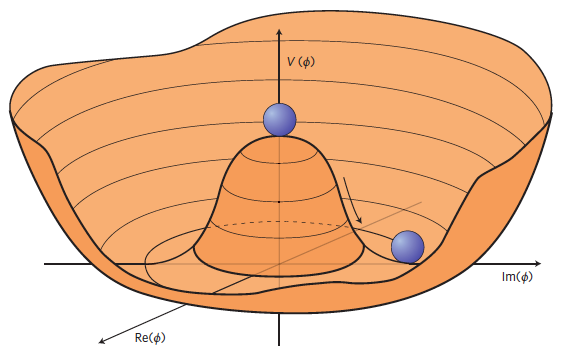
\includegraphics[width=0.65\linewidth]{figs/02_theory/higgspotential.png}
	\caption[The complex scalar potential for $\lambda^2>0$ and $\mu^2>0$, showing an infinite number of minima away from 0~\cite{higgspotential}. By inspection this potential possesses a global $U(1)$ gauge invariance due to the rotational symmetry from adding a complex phase.]{The complex scalar potential for $\lambda>0$ and $\mu^2>0$, showing an infinite number of minima away from 0~\cite{higgspotential}. By inspection this potential possesses a global $U(1)$ gauge invariance due to the rotational symmetry from adding a complex phase.}
	\label{fig:higgs_ssb}
\end{figure}

Without loss of generality, the global minimum can be chosen at $(\frac{\mu}{\lambda},0)$ and the fields can be expanded around the minimum as $\phi_1(x)=\eta(x)+\frac{\mu}{\lambda}$ and $\phi_2(x)=\xi(x)$. The Lagrangian can be written in these terms as
\begin{equation}
	\mathcal{L}=\underbrace{\frac{1}{2}(\partial_\mu\eta)(\partial^\mu\eta)-\mu^2\eta^2}_\text{Massive scalar field}+\underbrace{\frac{1}{2}(\partial_\mu\xi)(\partial^\mu\xi)}_\text{Massless scalar field}-\underbrace{\mu\lambda(\eta^3+\eta\xi^2)+\frac{\lambda^2}{4}(\eta^4+\xi^4+2\eta^2\xi^2)}_\text{Interaction terms} + \underbrace{\frac{\mu^4}{4\lambda^2}}_\text{Constant}
\end{equation}
Without adding any additional terms, the original Lagrangian now shows a massive scalar field $\eta$ with mass $m_\eta=\sqrt{2}\mu$ and a massless scalar field $\xi$. This massless field is known as a Goldstone boson and is a general feature of spontaneous symmetry breaking~\cite{goldstone}.

Following the prescription in section~\ref{sec:sm_theory_gauge}, we promote the global $U(1)$ symmetry to a local symmetry with $\phi\to\phi'=e^{ig\theta(x)}\phi$. The derivatives are replaced by covariant derivatives $\partial_\mu\to D_\mu=\partial_\mu+igB_\mu$, and we add the kinetic term from the Proca Lagrangian $-\frac{1}{16\pi}F^{\mu\nu}F_{\mu\nu}$. The new vector field $B_\mu$ transforms in the usual way $B_\mu\to B_\mu'=B_\mu-\partial_\mu\theta(x)$. Once again expanding in terms of $\eta$ and $\xi$, the gauge invariant Lagrangian becomes
\begin{align}
	\begin{split}
	\mathcal{L}=&\underbrace{\frac{1}{2}(\partial_\mu\eta)(\partial^\mu\eta)-\mu^2\eta^2}_\text{Massive scalar field}+\underbrace{\frac{1}{2}(\partial_\mu\xi)(\partial^\mu\xi)}_\text{Massless scalar field}-\underbrace{\mu\lambda(\eta^3+\eta\xi^2)+\frac{\lambda^2}{4}(\eta^4+\xi^4+2\eta^2\xi^2)}_\text{Interaction terms}\\
	&+\frac{\mu^4}{4\lambda^2}-\underbrace{\frac{1}{16\pi}F^{\mu\nu}F_{\mu\nu}+\frac{1}{2}\left(\frac{g\mu}{\lambda}\right)^2B_\mu B^\mu}_\text{Massive vector field}+g\frac{\mu}{\lambda}(\partial_\mu\xi)B^\mu
	\end{split}
\end{align}
As with before, the Lagrangian now shows a massive scalar field $\eta$, Goldstone boson $\xi$, and interaction terms between the scalar fields. The promotion from global to local gauge invariance has created a \textit{massive} vector field $B_\mu$ with $m_B=2\sqrt{\pi}g\mu/\lambda$ and a term coupling $B_\mu$ to $\xi$. The term coupling $B_\mu$ to $\xi$ allows the spin-1 vector field to transform into a spin-0 scalar field, which is non-physical and suggests that a gauge transformation is required to obtain the physical fields. It is possible to transform away the massless $\xi$ field entirely by taking $\theta(x)=\frac{\xi(x)}{g\mu/\lambda}$, which gives
\begin{align}
	\begin{split}
		\mathcal{L}\to\mathcal{L'}=&\left[\frac{1}{2}(\partial_\mu\eta)(\partial^\mu\eta)-\mu^2\eta^2\right]+\left[-\frac{1}{16\pi}F^{\mu\nu}F_{\mu\nu}+\frac{g}{2}\frac{\mu^2}{\lambda^2}B_\mu B^\mu\right]\\
		&+g^2\frac{\mu}{\lambda}\eta B^\mu B_\mu+g^2\frac{1}{2}\eta^2B^\mu B_\mu-\lambda\mu\eta^3-\frac{\lambda^2}{4}\eta^4+\frac{\mu^4}{4\lambda^2}
	\end{split}
\end{align}
After the gauge transformation, the Goldstone field has vanished from the Lagrangian, and the vector field $B_\mu$ gained additional terms corresponding to its longitudinal polarization along $\eta$ (colloquially, it is said the $B_\mu$ field ``ate'' the Goldstone boson). This gauge is referred to as the \textit{unitary} gauge.

It may seem counter-intuitive that a local $U(1)$ gauge transformation can alter a Lagrangian that was explicitly constructed to be invariant under local $U(1)$ gauge transformations, but this is the core principle of spontaneous symmetry breaking. The Lagrangian has inherent symmetry, but by decomposing the fields into the longitudinal and transverse components at a non-zero vacuum expectation value, the field variables themselves no longer display this symmetry. In this way, the physical fields are revealed to be a massive spin-0 field and massive spin-1 field, with the Goldstone boson absorbed into the spin-1 field.

\subsection{The Higgs Mechanism} \label{sec:sm_theory_beh}
In the previous section, we derived the Lagrangian for a broken $U(1)$ symmetry. In this section, the concepts of spontaneous symmetry breaking will be applied to the electroweak gauge symmetry $SU(2)_L\otimes U(1)_Y$. The simplest model of the Higgs field is an isospin doublet with one neutral component $\phi^0$ and a charged component $\phi^+$. The field can be written as
\begin{equation}
	\phi=\begin{pmatrix}\phi^+\\\phi^0\end{pmatrix}=\frac{1}{\sqrt{2}}\begin{pmatrix}\phi_1+i\phi_2\\\phi_3+i\phi_4\end{pmatrix}
\end{equation}
with a Lagrangian given by
\begin{equation}
	\mathcal{L}=(\partial_\mu\phi)^\dagger(\partial^\mu\phi)-V(\phi) \qquad V(\phi)=-\mu^2\phi^\dagger\phi+\lambda^2(\phi^\dagger\phi)^2
\end{equation}
with the assumption that $\lambda^2>0$ and $\mu^2>0$ necessary for spontaneous symmetry breaking.  The doublet has a set of global minimum defined by $\phi^\dagger\phi=\frac{\mu^2}{2\lambda^2}$, meaning the vacuum expectation value is $\left<\phi\right>_0=\frac{\mu}{\sqrt{2}\lambda}$.

To simplify the Lagrangian, it is helpful to start with the Higgs field $\phi$ already transformed to the unitary gauge. For any doublet $\phi$, there exists some global $SU(2)$ transformation $\hat{U}$ that rotates the doublet as follows
\begin{equation}
	\phi\to\phi'=\hat{U}\frac{1}{\sqrt{2}}\begin{pmatrix}\phi_1+i\phi_2\\\phi_3+i\phi_4\end{pmatrix}=\frac{1}{\sqrt{2}}\begin{pmatrix}0\\\tilde{h}(x)\end{pmatrix}
\end{equation}
such that $\tilde{h}(x)$ is entirely real valued~\cite{mandl2010quantum}. The specific form of $\hat{U}$ is unimportant for this derivation, all we require is that some $\hat{U}$ exists. We choose the global minimum to be $\frac{1}{\sqrt{2}}\begin{pmatrix}0\\\mu/\lambda\end{pmatrix}$ and expand $\tilde{h}(x)$ around this minimum as $\tilde{h}(x)=\frac{\mu}{\lambda}+h(x)$.

We are interested in the mass terms for the scalar boson, which originate from the covariant derivative terms as shown in the $U(1)$ example in section~\ref{sec:sm_theory_ssb}. Using the covariant derivative from equation~\ref{eq:ew_cov_derivative}, we get
\begin{equation}
	\partial_\mu\phi\to D_\mu\phi=\partial_\mu\phi+ig\boldsymbol{\tau}\cdot\mathbf{W}_\mu\phi+ig'\frac{1}{2}YB_\mu\phi
\end{equation}
The lower doublet has charge 0 and weak isospin $I^3=-\frac{1}{2}$, therefore has hypercharge $Y=2(Q-I^3)=1$. The full covariant derivative is then
\begin{align}
	\begin{split}
		D_\mu\phi&=\frac{1}{2\sqrt{2}}\begin{pmatrix}2\partial_\mu+igW_\mu^3+ig'B_\mu&ig(W_\mu^1-iW_\mu^2)\\ig(W_\mu^1+iW_\mu^2)&2\partial_\mu-igW_\mu^3+ig'B_\mu\end{pmatrix}\begin{pmatrix}0\\\frac{\mu}{\lambda}+h(x)\end{pmatrix}\\
		&=\frac{1}{2\sqrt{2}}\begin{pmatrix}\left[ig(W_\mu^1-iW_\mu^2)\right]\left(\frac{\mu}{\lambda}+h(x)\right)\\\left(2\partial_\mu-igW_\mu^3+ig'B_\mu\right)\left(\frac{\mu}{\lambda}+h(x)\right)\end{pmatrix}\\
	\end{split}
\end{align}
with the full expression given by
\begin{align}
	\begin{split}
		\left(D_\mu\phi\right)^\dagger\left(D^\mu\phi\right)=&\frac{1}{2}\left(\partial_\mu h(x)\right)\left(\partial^\mu h(x)\right)+\frac{1}{8}g_W^2\left(W_\mu^{(1)}+iW_\mu^{(2)}\right)\left(W^{(1)\mu}-iW^{(2)\mu}\right)\left(\frac{\mu}{\lambda}+h(x)\right)^2\\
		&+\frac{1}{8}\left(gW_\mu^{(3)}-g'B_\mu\right)\left(gW^{(3)\mu}-g'B^\mu\right)\left(\frac{\mu}{\lambda}+h(x)\right)^2
	\end{split}
\end{align}
The mass terms, which are proportional to the quadratic field terms, can be extracted as the following
\begin{equation}
	\mathcal{L}_\text{mass}=\frac{1}{8}(g\frac{\mu}{\lambda})^2\left(W_\mu^{(1)}W^{(1)\mu}+W_\mu^{(2)}W^{(2)\mu}\right)+\frac{1}{8}\left(\frac{\mu}{\lambda}\right)^2\left(gW_\mu^{(3)}-g'B_\mu\right)\left(gW^{(3)\mu}-g'B^\mu\right)
\end{equation}
The mass of the $W^1$ and $W^2$ fields can be identified immediately from the first term as $m_W=\frac{1}{2}g\frac{\mu}{\lambda}$. For the second term, it is apparent that there will be some combination of the $W_\mu^{(3)}$ and $B_\mu$ fields that result in a quadratic field term. Using the change of basis transformation defined in equation~\ref{eq:ew_mixing}, the last mass term transforms to
\begin{equation}
	\frac{1}{8}\left(\frac{\mu}{\lambda}\right)^2(g^2+g'^2)Z_\mu Z^\mu
\end{equation}
with a mass given by $m_Z=\frac{1}{2}\frac{\mu}{\lambda}\sqrt{g^2+g'^2}$. This $Z_\mu$ field can be identified as the \PZ boson. The remaining field $A_\mu$ remains massless and represents the photon. Thus, the Higgs mechanism results in the three massive gauge bosons and a massless photon.

In section~\ref{sec:sm_theory_ew} it was shown that the fermion mass must be 0, as the $\bar{\psi}_L\psi_R$ terms transform differently under local $SU(2)\otimes U(1)$ gauge transformations. Now we can consider the Yukawa Lagrangian, in which the fermions are coupled to the Higgs field $\phi$. Using the first generation leptons as an example, the Yukawa Lagrangian reads
\begin{equation}
	\mathcal{L}=-g\left(\bar{\chi}_L\phi e_R+\bar{e}_R\phi^\dagger\chi_L\right)
\end{equation}
For an $SU(2)$ transformation $\hat{U}(x)$, the quantity $\bar{\chi}_L\phi$ transforms as
\begin{equation}
	\bar{\chi}_L\phi\to\bar{\chi}'_L\phi'=\bar{\chi}_L\hat{U}^*(x)\hat{U}(x)\phi=\bar{\chi}_L\phi
\end{equation}
Since $\left(\phi^\dagger\chi_L\right)^\dagger=\bar{\chi}_L\phi$, the Yukawa Lagrangian is invariant. By using the Higgs field in the Unitary gauge, the Yukawa Lagrangian can be explicitly written as
\begin{align}
	\begin{split}
		\mathcal{L}&=-\frac{g}{\sqrt{2}}\left[\begin{pmatrix}\PAGne&\PAe\end{pmatrix}_L\begin{pmatrix}0\\\frac{\mu}{\lambda}+h(x)\end{pmatrix}\Pe_R+\PAe_R\begin{pmatrix}0&\frac{\mu}{\lambda}+h(x)\end{pmatrix}\begin{pmatrix}\PGne\\\Pe\end{pmatrix}_L\right]\\
		&=-\frac{g}{\sqrt{2}}\frac{\mu}{\lambda}(\PAe_L\Pe_R+\PAe_R\Pe_L)-\frac{g}{\sqrt{2}}h(x)(\PAe_L\Pe_R+\PAe_R\Pe_L)\\
		&=-m_e\PAe\Pe-\frac{m_e}{\mu/\lambda}\PAe\Pe h(x)
	\end{split}
\end{align}
where the mass of the electron has been identified from the first term as $m_e=\frac{g}{\sqrt{2}}\frac{\mu}{\lambda}$. The second term shows that the fermion coupling to the Higgs field is proportional to the fermion mass. Note that this Lagrangian only selects the lower $I^3=-\frac{1}{2}$ fermion from the left-handed doublets. To apply this method for the $I^3=+\frac{1}{2}$ fermions, the Higgs field is replaced by its charge conjugate $\phi_c$ given by
\begin{equation}
	\phi_c=-i\sigma_2\phi^*=\frac{1}{\sqrt{2}}\begin{pmatrix}-\frac{\mu}{\lambda}-h\\0\end{pmatrix}
\end{equation}
and the charge conjugate Lagrangian for a fermion $f$ is given as $\mathcal{L}_c=g_f[\chi_L\phi_cf_R+\bar{f}_R\phi_c^\dagger\chi_L]$. It is this Yukawa Lagrangian that provides the masses to the fermions and couples them to the Higgs field.

\section{Fermi's Golden Rule and Particle Lifetimes}
One of the key results from QFT relates the interactions between particles to the rate at which they decay. Fermi's Golden Rule, which is more commonly known from perturbation theory in QM, can be applied to Lorentz invariant particle decays~\cite{pdg2024}. For the decay $1\to2+3+...+n$, the partial decay rate is given by
\begin{equation}
	d\Gamma=\frac{(2\pi)^4}{2m_1}|\mathcal{M}|^2d\Phi_n(p_1,p_2,...,p_n)
\end{equation}
where $\mathcal{M}$ is the matrix element of the decay determined by the coupling constant and the interaction term of the initial and final states in the Lagrangian and $d\Phi_n(p_1,p_2,...,p_n)$ is a differentiable element of the phase space given by
\begin{equation}
	d\Phi_n(p_1,p_2,...,p_n)=\delta^4(p_1-\sum_{i=2}^n p_i)\prod_{i=2}^n\frac{d^3p_i}{(2\pi)^32E_i}
\end{equation}
For a two body decay, integrating over the phase space gives a total decay rate of
\begin{equation}
	\Gamma=\frac{|p_i|}{8\pi m_1^2}|\mathcal{M}|^2
\end{equation}
This is the total decay rate for the specific process $1\to2+3$. One parameter of interest is the total decay rate for all processes, given by $\Gamma=\sum_{i}\Gamma_i$, where $i$ sums over all possible decay modes. Particles decays are a Poisson process, meaning that the decay probability is independent of how long the particle has existed. Given $N$ particles, the expected remaining after a time $t$ would therefore follow an exponential distribution given by
\begin{equation}
	N(t)=N_0e^{-\Gamma t}
\end{equation}
The mean lifetime would then be given by $\tau=1/\Gamma$.
\section{Motivations for Long Lived Scalar Bosons} \label{sec:BSM}
Despite the standard model's success as the most accurate and precise description of fundamental particles and their interactions, there exist substantial shortcomings that remain unanswered. 